\documentclass[b5paper,11pt]{article}
\bibliographystyle{plain}

\usepackage{geometry}
\usepackage{amssymb,amsthm,bm,mathrsfs,mathtools}
\usepackage[usenames]{xcolor}
\usepackage{hyperref}
\usepackage{graphicx,subcaption}
\graphicspath{{../"img/"}{../"figures/"}}

\usepackage{mycommands}
\newcommand{\numcircled}[1]{\raisebox{.5pt}{\textcircled{\raisebox{-.9pt} {#1}}}}
\newcommand{\Dmax}{\trdis_\mathsf{max}}
\newcommand{\InFmax}{\infid_\mathsf{max}}
\newcommand{\Psb}{\mathcal{P}_\mathrm{SB}}
\newcommand{\Odd}{\Omega_{\mathsf{DD}}}
\newcommand{\Opdd}{\Omega_{\mathsf{PDD}}}
\newcommand{\vOpdd}{\vec{\Omega}_{\mathsf{P}}}
\newcommand{\LO}[1]{\operatorname{LO}}

\newcommand{\wt}[1]{\widetilde{#1}}

\newcommand{\Heff}{H_\mathrm{eff}}
\newcommand{\HeffB}{H_\mathrm{eff,B}}
\newcommand{\HeffSB}{H_\mathrm{eff,SB}}

\newcommand{\CDDn}{\mathrm{CDD}_n}
\newcommand{\rDD}{\mathrm{DD}}
\newcommand{\rmax}{\mathrm{max}}
\begin{document}
\subsection{Note on noisy gates}
Previously, we treated the DD control gates in an ideal manner, which implies instantaneous and noise-free pulses. In practice, of course, the control gates are neither instantaneous nor noise-free. Hence the analysis for ideal DD cannot be directly carried out.

The effects of quantum noise on the system can be generally modelled with CPTP channels, which need not be unitary. The introduction of non-unitarity is problematic as the error phase, which is used to study the efficacy of DD, can no longer be defined.
However, one may include some ancillary qubits to transform any quantum channel into a unitary evolution over the extended Hilbert space. For the analytical treatment below, we will always assume this dilation for the noisy gates. As a result, we can ascribe Hamiltonian generators for the noisy control gates. 
The Hamiltonian can be time-dependent and involves in both the environment coupling and gate control.
Focusing on the $i$th gate-interval,  we can write the total Hamiltonian:
\begin{equation}\label{eq:noisy-Hamiltonian}
 H(t) = H_e + H_c(t), \quad t_{i-1}< t \le t_i,
\end{equation}
where $H_e=H_\rB+H_\rSB$ is the error Hamiltonian between system and bath;
and $H_c(t)$ is the applied control Hamiltonian.
For simplicity, we also assume that $H_c(t)$ is 
only dependent on the control gate it aims to perform, and is irrelevant to the 
particular execution time/order of the gate.



The perfect control Hamiltonian, which we considered earlier, is a delta spike  at $t=t_i$ that generates the exact $P_i$-gate.  In reality, the control Hamiltonian $H_c(t)$ is not a delta spike and will be prone to error. The results for the ideal DD case can no longer be directly applied. 
Directly solving the time evolution operator $U(T,0)$ from $H(t)$ is also impractical, as the very large $H_c(t)$ integral will break the convergence conditions for typical approximation methods. To correctly estimate the time evolution, it is necessary to separate out the strong ``gate parts'' from the weak ``noise parts''. 
We force such separation by formally expressing the time evolution operator according to \Eqref{eq:noisy-Hamiltonian} as:
\begin{equation}\label{eq:noisy-gate-formal}
U(t_{i},t_{i-1})=
 P_i \exp(-\upi \wt\Omega_{P_i}) \equiv \wt U_{P_i}, 
\end{equation}
where we put tildes over the characters to distinguish the noisy DD against the ideal DD case. 
Here the noise generator $\wt\Omega_{P_i}$ associated with $\wt U_{P_i}$ replaces  $\Omega$ for the ideal $U_{P_i}$. 
Similar to the ideal DD case, we can split the decoupling gates by defining $P_i=G_{i+1}^\dagger G_{i}$ and then,
\begin{equation}
  U(T,0) = \upe^{-\upi  G_L \wt\Omega_{P_L}  G_L^\dagger} \ldots
  \upe^{-\upi G_1\wt\Omega_{P_1}G_1^\dagger} 
  \equiv \wt U_\rDD \equiv\upe^{-\upi\wt\Omega_\rDD} .
\end{equation}
For weak system-environment coupling and small gate error,  $\wt\Omega_{P_i}$s are in the vicinity of zero.
We may then use the Magnus formula to derive the leading order Magnus series as good approximation to $\wt\Omega_\rDD$.

The overall goal is to figure out sufficient conditions such that the noise-inflicted DD error phase $\wt\Phi_\rSB \equiv \norm{\wt\Omega_{\rDD,\rSB}}$  is still reduced compared to the bare Hamiltonian error phase $\phi_\rSB = \norm{\Omega_{\rSB}}$.
 In this paper, we mainly focus on the breakeven conditions for PDD and CDD. But our analysis should be easily generalized to other DD schemes as well.
For the $X$-gate and $Z$-gate required for PDD and CDD, let us 
associate the generic gate-dependent noise as:
\begin{equation}\label{eq:gatedep-noise}
\wt U_X= X \upe^{-\upi \wt\Omega_X},
\quad \wt U_Z= Z \upe^{-\upi \wt\Omega_Z}.
\end{equation}
The PDD time evolution map is simplicity $\wt U_\sP =\wt U_Z \wt U_X \wt U_Z \wt U_X\equiv\upe^{-\upi \wt\Omega_\sP}$.
With these noisy gates substituted, the effective Hamiltonian
 can be solved through a Magnus series 
$\wt{\Omega}_{\sP} =\sum_n \wt{\Omega}_{\sP}\up{n}$. 
Supposing that $ \wt\Omega_X = \sum_i \sigma_i \otimes B'_i$ and 
$ \wt\Omega_Z= \sum_i \sigma_i \otimes B''_i$, we can explicit express the first two terms as:
\begin{align}\label{eq:PDDMagGatedep}
&\widetilde{\Omega}_\sP^{(1)} 
= \sigma_0 \otimes 2(B'_0 + B''_0) + \sigma_2 \otimes 2(B_2'-B_2''), \\
&\widetilde{\Omega}_\sP^{(2)} = \notag
\sigma_0 \otimes \upi\,([B'_0,B''_0]+\![B'_1,B''_1]-\![B'_2,B''_2]-\![B'_3,B''_3]) \\[0.5ex]
&\! + \sigma_1 \otimes 
(-\upi\,[B_0'{+}B_0'',B_1'{+}B_1'']+\{B_2'{-}B_2'', B_3'{-}B_3''\}) \notag \\[0.5ex]
 &\!+ \sigma_2 \otimes 
(-\upi\,[B_0',B_2'']\!-\upi\,[B_0'',B_2'] -\! \{B_1',B_3''\}
 -\!\{B_1'',B_3'\} ) \notag\\[0.5ex]
 &\!+\sigma_3 \otimes 
(\upi\,[B_0'{+}B_0'',B_3''{-}B_3'] + \{B_1'{+}B_1'',B_2''{-}B_2'\}).
\label{eq:PDD-gatedep-Mag2}
\end{align}
When $\wt\Omega_X=\wt\Omega_Z$, These two Magnus terms would recover the ideal PDD expression 
\Eqref{eq:PDDMagIdeal} as expected. Furthermore,  \Eqref{eq:PDDMagGatedep} suggests that the first order decoupling can be achieved as long as $B_2'=B_2''$.  With generic gate-dependent noise, 
however, the first order coupling no longer vanishes. In the case where $\wt\Omega_X$ and $\wt\Omega_Z$ are small and not correlated,
the error phase of the resulting PDD map will be dominated by the
first order term:
\begin{equation}
    \wt\Phi_{\rSB}\approx \norm{2(B_2'-B_2'') }.
\end{equation} 
Typically, the error phase of $\wt\Omega_X$ and $\wt\Omega_Z$ are at least on the same order as the free evolution one, $\phi_\rSB$.
Directly applying triangular inequality for the r.h.s.\ will produce the  upper-bound $4\phi_\rSB$. This rough estimation directly violates the breakeven condition. Hence, to derive the breakeven condition for noisy PDD, it is necessary to introduce more detailed models in which one can characterize the extra amount of noise introduced by the control. 
 For simplicity, let us employ a parameter $\eta$ for the noise strength, which is defined later.  The break-even condition is, in essence, to solve the inequality
$\wt\Phi_\rSB(\phi_\rB,\phi_\rSB,\eta) < \phi_\rSB$,
and obtain an upper bound on the noise level $\eta<\eta_{\rmax}(\phi_\rB, \phi_\rSB)$.
To achieve this, we not only need an appropriate noise strength parameter $\eta$, but also derive tighter upper-bound for the DD error phase function.




\subsection{Noisy pulses}
If the non-zero duration of $H_c(t)$ is much shorter than the gate interval,  the control gates can still be viewed as instantaneous pulses. In this section we consider such type of noise models. 
Specifically, we may view
$H_c(t)\sim \delta(t-t_i)$, but does not produce the ideal gate.
The time evolution operator for the $i$th gate interval becomes:
\begin{equation}\label{eq:npulses-Ui}
 \wt U_{P_i} = \wt P_i \upe^{-\upi \Omega},
\end{equation}
where $\widetilde{P}_i \equiv\upe^{-\upi \int H_c(t) \dd t}\neq P_i$ is the noisy $P_i$ gate and $\Omega=\tau H_e$ is the free evolution generator.
The Hermitian generator associated with $\wt P_i$  should be dominated by that of an ideal gate in addition to a small noise part:
\begin{equation}\label{eq:npulses-Pi}
 \widetilde{P}_i= \exp\left[ -\upi \left( \Omega_{P_i} +  \eta \Gamma_{P_i} \right)  \right],
\end{equation}
where $\Omega_{P_i}$ is responsible for the ideal gate $P_i = \exp(-\upi \Omega_{P_i})$ and supported only on the system; and $ \eta \Gamma_{P_i} $ is responsible for the noise and supported on the system-bath-ancilla composite in general. We set $\max_j (\norm{\Gamma_{P_j}} )=1$ and employ the smallness parameter $\eta$ for order tracking. For the $X$-gate and $Z$-gate in particular, we consider:
\begin{equation}
\widetilde{X} = \upe^{-\upi ( \frac{\pi}{2} \sigma_1 + \eta\Gamma')},\quad
 \widetilde{Z} = \upe^{-\upi ( \frac{\pi}{2} \sigma_3 + \eta\Gamma'')},
\end{equation}
where $\Gamma'$ and $\Gamma''$ account for the extra noise 
in the $X$-gate and $Z$-gate and are explicit expressed as
 $\Gamma' = \sum_i \sigma_i \otimes B'_i $ and $\Gamma''=\sum_i \sigma_i \otimes B''_i$. 
The time evolution for the noisy PDD sequence then becomes
 \begin{align}
 \notag
\wt U_\rDD &=
 \widetilde{Z} \upe^{-\upi \Omega}
 \widetilde{X} \upe^{-\upi \Omega}
 \widetilde{Z} \upe^{-\upi \Omega}
 \widetilde{X} \upe^{-\upi \Omega} \\
 \label{eq:UPDD-gatedep}
 & = \upe^{-\upi  \Gamma_3} \upe^{- \upi\Omega_3}
 \upe^{-\upi  \Gamma_2}  \upe^{-\upi\Omega_2}
\upe^{-\upi  \Gamma_1} \upe^{-\upi\Omega_1}
\upe^{-\upi  \Gamma_0}  \upe^{-\upi \Omega_0}, 
\end{align}
where $\Omega_i \equiv \sigma_i \Omega \sigma_i$ as already appeared in 
 the ideal case; and we have further introduced
$\upe^{-\upi  \Gamma_3}=\wt Z Z$, 
$\upe^{-\upi  \Gamma_2}=Z \wt X Y$,
$\upe^{-\upi  \Gamma_1}=Y \wt Z X$ and 
$\upe^{-\upi  \Gamma_0}=X \wt X$.
By keeping the leading order in 
$\eta$, we can estimate these operators as:
\begin{equation}
 \begin{aligned}
  \Gamma_3 &= \eta(\sigma_0 \otimes B_0''- \frac{2}{\pi} \sigma_1 \otimes B_2'' 
  +\frac{2}{\pi}  \sigma_2 \otimes B_1'' + \sigma_3 \otimes B_3''),\\
  \Gamma_2 &= \eta(\sigma_0 \otimes B_0'- \sigma_1 \otimes B_1'
  +\frac{2}{\pi}  \sigma_2 \otimes B_3' + \frac{2}{\pi} \sigma_3 \otimes B_2'),\\
  \Gamma_1 &= \eta(\sigma_0 \otimes B_0''+ \frac{2}{\pi} \sigma_1 \otimes B_2'' 
  +\frac{2}{\pi}  \sigma_2 \otimes B_1'' - \sigma_3 \otimes B_3''),\\
  \Gamma_0 &= \eta(\sigma_0 \otimes B_0'+ \sigma_1 \otimes B_1'
  +\frac{2}{\pi}  \sigma_2 \otimes B_3' - \frac{2}{\pi} \sigma_3 \otimes B_2').
 \end{aligned}
\end{equation}
As every exponent in \Eqref{eq:UPDD-gatedep}  is small, we can apply the Magnus formula to calculate $\widetilde\Omega_\mathrm{PDD}$. 
The first order Magnus term suggests:
\begin{equation}
 \wt\Omega_\rDD\up{1}= \sigma_0 \otimes (4B_0 + 2\eta( B'_0 + B''_0)) 
+ \sigma_2 \otimes \frac{4}{\pi}\eta(B_1''+B_3').
\end{equation}
The term that acts non-trivially on the system is proportional to $B_1''+B_3'$. 
Assuming $B_1''+B_3'\neq 0$,  exact first order decoupling is lost. 
When the gate noise strength $\eta$ is at least of similar size as $\phi_\rSB$---the gate noise typically dominates the background noise in many experiments---the first order Magnus term would be of leading order in magnitude. And the error phase after PDD is reduced to a linear multiple in $\eta$. 
 we upper-bound the size of the first order coupling by:
\begin{equation}
 \wt\Phi_\rSB \approx \norm{ \frac{4\eta}{\pi}(B_1''+B_3')} \le \frac{8}{\pi}\eta.
\end{equation}
This results in the first order breakeven condition:
\begin{equation}
 \eta \le \frac{\pi}{8} \phi_\rSB.
\end{equation}
This condition indicates that in order to achieve noise suppression, the gate noise should be bounded by a fraction of the free evolution noise. Hence, if any improvement from DD is expected, the control pulses must be very accurate in the first place. 
On the other hand if $\eta\ll \phi_\rSB$, the existence of pulse noise contributes negligibly and the second oder term will be similar to the ideal PDD case. Hence to faithfully approximate the full $\wt\Omega_\rDD$, we may keep every term that is linear in $\eta$ and up to second order in the smallness $\phi$. Focusing on the interaction part, the result becomes:
\begin{equation}
 \wt\Omega_{\rDD:\rSB} = \Omega_{\rDD:\rSB} +\sigma_2 \otimes \frac{4}{\pi}\eta(B_1''+B_3') + \cO(\eta\phi,\phi^3),
\end{equation}
where $\Omega_{\rDD:\rSB}$ is the interaction part for the ideal PDD, whose norm is bounded by $\norm{\Omega_{\rDD:\rSB}} \le \Phi_\rSB^{(\mathrm{ub})}$ 
as we have already calculated.
Applying triangular inequality and bounding the resulting error phase by $\phi_\rSB$, we reach the more rigorous second order breakeven condition:
\begin{equation}\label{eq:npulses-breakeven2}
   \eta \le \frac{\pi}{8} \phi_\rSB - \frac{\pi}{8}\Phi_\rSB^{(\mathrm{ub})}.
\end{equation}
We remark that this is a loose bound and tighter bound can be obtained by performing optimization on $\norm{\wt\Omega_{\rDD:\rSB}}$ akin to what we did for the ideal case, rather than using triangular inequality. But the current form is enough to serve our purpose.

To verify our results, we numerically simulated PDD with noisy pulses and compare the data with our our breakeven conditions in \Figref{fig:pdd-noisy-pulse}. 
Specifically, for each fixed tuple of parameters $(\phi_\rB,\phi_\rSB,\eta)$, we randomly generate 300 sets of the Hermitian matrices $\{\Omega,\Gamma',\Gamma''\}$
satisfying the given parameters over a uniform distribution. Noisy PDD is simulated for each particular set of  bare Hamiltonian and noisy pulses; the noise reduction ratio $\wt\Phi_\rSB/\phi_\rSB$ is obtained and numerically maximized for the fixed $(\phi_\rB,\phi_\rSB,\eta)$. 
We used two figures to visualize the effect of noisy pulses. First is the deformation---or shrinking to be exact---of the noise removal region in the $(\phi_\rB,\phi_\rSB)$ phase diagram. Second is the dependence between the maximally allowed noise versus the free-evolution noise. From the figure we can see that our first order condition works well as long as the noise parameter $(\phi_\rB,\phi_\rSB)$ is weak and the second order condition is more universally applicable for a wider range of conditions.



 \begin{figure}
 \centering
 \begin{subfigure}{0.45\linewidth}
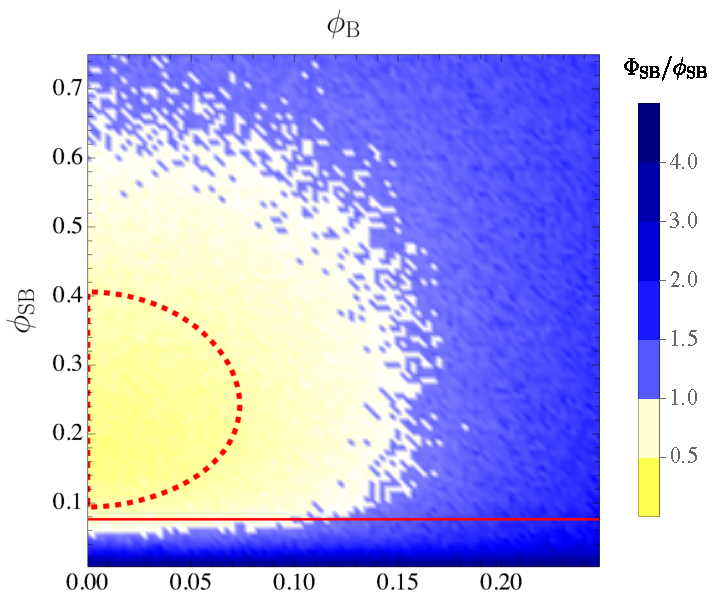
\includegraphics[height=0.8\linewidth]{pdd-noisypulse1}
\caption{$\eta =0.03$.}
\label{fig:pdd-noisy-pulse1}
\end{subfigure}
\hfill
\begin{subfigure}{0.45\linewidth}
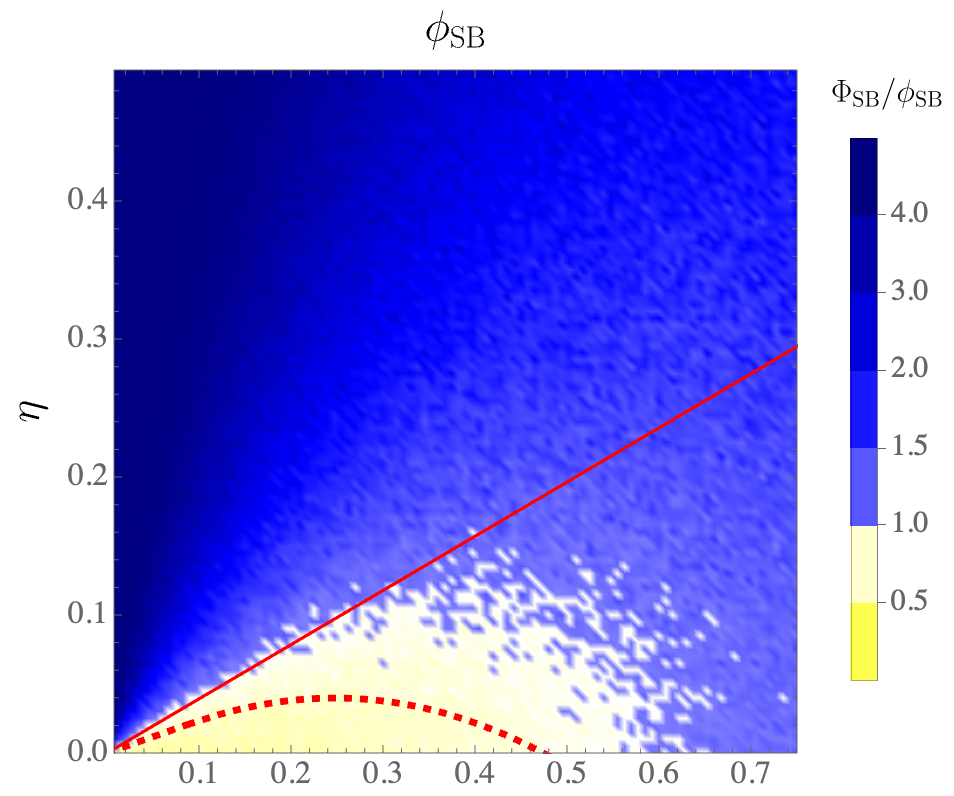
\includegraphics[height=0.8\linewidth]{pdd-noisypulse2}
\caption{$\phi_\rB =0.05$.}
\label{fig:pdd-noisy-pulse2}
\end{subfigure}
\caption{The maximal noise reduction ratio for the noisy PDD. A point is colored yellow if the noise is reduced after PDD.  The first order condition is indicated with the red solid line while the second order condition is indicated with the red dashed line. }
\label{fig:pdd-noisy-pulse}
\end{figure}



We now examine the special scenario where the first order decoupling is exact, which requires $B''_1+B'_3=0$. It can be shown that this condition actually corresponds to a ``weakly gate-dependent'' noise model:
\begin{equation}\label{eq:gateindep1}
 \wt P_i = P_i \upe^{-\upi \eta \Gamma + \cO(\eta^2)},\ \forall i.
\end{equation}
For the most generic noisy pulses, we can write introduce the gate-noise decomposition $\wt P_i = P_i \upe^{-\upi \eta \Gamma_i}$. The weak gate-dependence assumption is demanding that the variance in $\Gamma_i$  
is at most on the order of the smallness parameter $\eta$.
 That is, the dependence of the noise on the gate is weak. If this condition is 
 satisfied, then the time evolution readily reduces to the ideal DD case by replacing $\Omega=\tau H$ for free evolution with an effective Hamiltonian $\wt\Omega$ such that
\begin{equation}
\upe^{-\upi \wt\Omega}=\upe^{-\upi \eta \Gamma}\upe^{-\upi \Omega}.
\end{equation}
Since $\Gamma$ and $\Omega$ are both small, as required for DD to work,
one may invoke the BCH formula to get $\wt\Omega$ as a series of nested commutators. 
The already established map $\Omega\to \Omega_{\rDD}$ for the idea-pulse DD sequence can then be reused to estimate $\Omega_{\rDD}$
Naturally, we recover exact first order decoupling for PDD. To derive the break-even condition for such weakly gate-dependent noise, 
we retain the BCH series to the second order term, and then apply triangular inequality to derive the upper bounds for $(\widetilde\phi_\rB,\widetilde{\phi}_\rSB) \equiv( \norm{\wt\Omega_\rB}, \norm{\wt\Omega_\rSB})$:
\begin{equation}\label{eq:comb-bound}
\left\{
\begin{aligned}
 \widetilde\phi_\rB &\lesssim (\eta + \phi_\rB)(1+\eta + \phi_\rSB) \equiv \widetilde\phi_\rB^{(\mathrm{ub})}\\
 \widetilde\phi_\rSB &\lesssim (\eta + \phi_\rSB) (1+\eta + \phi_\rB)\equiv \widetilde\phi_\rSB^{(\mathrm{ub})}
\end{aligned}
\right..
\end{equation}
With this, we can bound the error phase relevant for this noisy-pulse situation under the different schemes by replacing $\phi_\rB$ and $\phi_\rSB$ for the ideal case with their noisy upper bounds: 
\begin{equation}
 \widetilde\Phi_\rSB \le \Phi_\rSB(\widetilde\phi_\rB^{(\mathrm{ub})}  ,\widetilde\phi_\rSB^{(\mathrm{ub})} ) < \phi_\rSB.
\end{equation}
Further bounding the right hand side by $\phi_\rSB$ then gives us the condition for the break-even points.

The above analysis is generic and applies to all DD schemes with gate-independent noise. 
The resulting bound is general, but could be suboptimal for a specific DD scheme and a specific type of pulse imperfection. Below, we examine a concrete examples of imperfections  for PDD: 
global unitary error in the control gates,  which results in the noisy pulse 
\begin{equation}
\widetilde P_i=P_i\upe^{-\upi \bm{\theta}\cdot\bm\sigma},\ \forall i.
\end{equation}
We use the notation $\bm\sigma=(\sigma_1,\sigma_2,\sigma_3)$, and $\bm\theta\equiv (\theta_1,\theta_2,\theta_3)$ with $\theta_i$ real constants---taken as small for weak noise---that parameterize the unitary error.  This can arise from, for example, a systematic calibration error in the pulse control leading to a consistent over or under rotation. In this situation, $\Gamma\equiv \bm\theta\cdot\bm\sigma$ acts only on the system and does not have a pure bath term. In the appendix, we derive an tighter bound:
\begin{equation}\label{eq:eff-Hami-tcp}
\left\{
\begin{aligned}
\widetilde{\phi}_\rB &\le \phi_\rB + \frac{1}{3}\theta  \phi^2_\rSB  \\
\widetilde{\phi}_\rSB &\le \phi_\rSB +  \theta^2  \phi_\rSB  \\
\end{aligned}    \right.,
\end{equation}
where $\theta \equiv \norm{\bm \theta}$ is the rotation angle associated with the gate error.
Assuming the noise to be small, we may only use the leading order 
approximation, which is by itself accurate to the second order. 
Substituting the upper bounds to  $\Phi_\rSB(\wt\phi_\rB,\wt\phi_\rSB)$ and keeping the leading order terms,  we can predict the following simplified bound for PDD:
\begin{equation}\label{eq:npdd-bound-simple}
2\phi_\rB^2 + \frac{(\theta+\phi_\rSB)^4}{4\phi_\rSB^2}\le \frac{1}{16},
\end{equation}
From this inequality, the globally maximally allowed $\theta$ can be found at $\phi_\rB=0$, $\phi_\rSB=1/8$ with
$\theta_\mathrm{max}= 1/8$. Furthermore, we can solve for $\theta$ in terms of $\phi_\rB$ and $\phi_\rSB$ to arrive at the noise threshold for the rotation angle:
\begin{equation}\label{eq:npdd-err-thres}
    \theta \le (1-32\phi_\rB ^2)^{\frac{1}{4}} \sqrt{\frac{\phi_\rSB}{2} }-\phi_\rSB
    \quad \lesssim \sqrt{\frac{\phi_\rSB}{2}}.
\end{equation}
It states that for the regime where the the free evolution noise is small, gate noise should at most be on the order of the square root of the free evolution noise. This  is quite different from the generic noise case where the upper bound dependence in $\phi_\rSB$ is linear. 


\subsection{Control signals of finite shapes}
In reality the control signals have finite strength hence non-zero durations.
This deviation from the delta function contributes to an extra source of noise, which adds to the free evolution noise and gate control error. 




The simplest example is that of the finite width rectangular pulses. Assuming the pulse duration is $\tau_p$, the Hamiltonian  for the $i$th gate interval is split into two constant pieces: $H=H_e+H_c$ for $t_i -\tau_p  < t \le t_{i}$ when the control is in applied, while $H=H_e$ for other times. 
A similar noise model was first considered in the original CDD paper~\!\cite{khodjasteh2007performance}. It fact, it can be easily transformed into the 
case of noisy pulses considered earlier by replacing the free evolution generator $\Omega$ with $ (1-(\tau_p/\tau)) \Omega$ and the pulse noise generator $\eta \Gamma_{P_i}$ in \Eqref{eq:npulses-Pi} with $(\tau_p/\tau) \Omega$. In terms of PDD, to obtain the Magnus series for the finite width scenario, all we need is to make the substitutions $B_i \to (1-(\tau_p/\tau)) B_i$, $\eta B_i' \to (\tau_p/\tau) B_i$ and $\eta B_i'' \to (\tau_p/\tau) B_i$. Using the first order expansion, we estimate the error phase as 
\begin{equation}
\norm{ \wt\Omega_{\rDD:\rSB}\up{1} }\le \frac{4\sqrt{2}}{\pi} (\frac{\tau_p}{\tau})\phi_\rSB.
\end{equation}
We see that the error phase contribution from the finite width is automatically on the second order smallness if we assume $\tau_p\ll \tau$. In comparison,
the control error considered previously contributes to the first order smallness. 
This suggests DD is relatively more tolerant to the finite width error. The finite-width model produces the breakeven condition.
\begin{equation}
 \tau_p/\tau \le \frac{\pi}{4\sqrt{2}}\approx 0.555.
\end{equation}
Notice that this condition is derived without any control noise in mind. It puts an upper bound on how 
fast we are allowed to perform DD even with perfect control. That is, the 
control signal should at least be ``pulse-like'' by allowing some time for the free evolution.



Extending beyond the simple rectangular signal model, we now consider a more generic situation where the control signal can be of arbitrarily shape while also accounting for the gate control error. After shifting the time origin for simplicity, the total Hamiltonian within a gate interval can be split into three parts:
\begin{equation}\label{eq:Hami-3parts}
 H(t)= H_g(t) +  H_e +  H_{ge}(t), \ 0\le t\le \tau,
\end{equation}
where $H_g(t)$ is the ``gate'' Hamiltonian, responsible for the perfect gate; 
$H_e$ is the system-bath coupling Hamilton responsible for the free evolution noise,
and $H_{ge}(t)$ is the gate error Hamiltonian responsible for the control error. It is assumed that the control signal $H_g(t)$ is pulse-like and much greater than the two noise terms when control is turned on.
We isolate the pure gate part by writing the time evolution as 
\begin{equation}
 U(\tau)=P_g \upe^{-\upi \wt \Omega_g},
\end{equation}
 where $P_g=U_g(\tau)$ is the gate unitary generated by $H_g(t)$.
The interaction picture Hamiltonian defined by
$\wt H(t)\equiv U_g^\dagger(t) (H_e + H_{ge} (t)) U_g(t)$ completes the time evolution operator $\upe^{-\upi \wt \Omega_g}$
at $t=\tau$. 
Since both $H_e(t)$ and $H_{ge}(t)$ are small, we can approximate $\wt \Omega_g$ by neglecting their higher order commutators:
\begin{equation}
 \wt \Omega_g \approx\! \int_0^\tau\!\! U_g^\dagger(t) H_e U_g(t) \dd t\, + \! \int_0^\tau\!\! U_g^\dagger(t) H_{ge}(t) U_g(t) \dd t.
\end{equation} 
We refer the first term in the above as the pulse shape term and the second term as the pulse error term. 

The pulse shape term is very dependent on the control signal $H_g(t)$. But anyway let us formally express the results as:
\begin{equation}
\int_0^\tau\!\! U_g^\dagger(t) H_e U_g(t) \dd t =\sigma_0 B_0  +  \left\{
 \begin{aligned}
   & \sigma_1 B_1' + \sigma_2 B_2'+\sigma_3 B_3',\ g=X;\\
    &\sigma_1 B_1'' + \sigma_2 B_2''+\sigma_3 B_3'',\ g=Z.
 \end{aligned}
 \right.
\end{equation}
To deal with the pulse error term,  we can bound it by
\begin{equation}
 \norm{\int_0^\tau\!\! U_g^\dagger(t) H_{ge}(t) U_g(t) \dd t} 
 \le  \int_0^\tau\!\! \norm{H_{ge}(t)} \dd t \equiv  \eta,
\end{equation}
where the small number $\eta$ absorbs any time-dependence of the control Hamiltonian.
Hence we may effectively replace the pulse error term with a gate-dependent error map $\eta \Gamma_g$, where $\Gamma_g$ is Hermitian and $\norm{\Gamma_g}\le 1$.
After plugging 



Here we consider the $X$ and $Z$ gates necessary for PDD and CDD.
The gate Hamiltonian responsible for the Pauli gate $P_g\ (g\in\{X,Z\})$ should be proportional to $\sigma_g$:
\begin{equation}
 H_g(t) = \frac{1}{2}\omega_g(t)\sigma_g,\quad g\in\{X,Z\},
\end{equation}
where the time-dependent function $\omega_g(t)$ specifies the shape of the pulse and satisfies the condition that its time integral $\theta_g(\tau)=\pi$, with $\theta_g(t)\equiv \int_0^t \omega_g(t') \dd t'$.
This constrain is necessary for the $U_g(t)$ generated by $H_g(t)$
to recover the ideal gate at $t=\tau$. Within $t=0$ and $\tau$ we have 
\begin{equation}
 U_g(t) = \cos\Bigl(\frac{\theta_g(t)}{2} \Bigr) I -\upi \sin\Bigl(\frac{\theta_g(t)}{2} \Bigr)\sigma_g,\quad
 g = X,Z.
\end{equation}
After conjugating $H_e\tau = \sum_i \sigma_i \otimes B_i$ with $U_g(t)$,
we can write the pulse shape term as:
\begin{equation}\label{eq:pshape-term}
\begin{aligned}
&\int_0^\tau\!\! U_g^\dagger(t) H_e U_g(t) \dd t =\sigma_0 B_0  + \\
 & \left\{
 \begin{aligned}
   & \sigma_1 B_1 + 
   \langle \cos\theta_X \rangle \bigl( \sigma_2  B_2 + 
   \sigma_3 B_3 \bigr)+ 
   \langle\sin\theta_X \rangle
    \bigl(\sigma_2 B_3 - \sigma_3 B_2\bigr),\ g=X;\\
    &\sigma_3 B_3  + \langle \cos\theta_Z \rangle \bigl( \sigma_1  B_1 + 
   \sigma_2 B_2 \bigr)+ 
   \langle\sin\theta_Z \rangle
    \bigl(\sigma_1 B_2 - \sigma_2 B_1\bigr),\ g=Z,
 \end{aligned}
 \right.
\end{aligned}
\end{equation}
where the average trig-functions are defined as:
\begin{equation}
 \langle \cos(\theta_g) \rangle \equiv \frac{1}{\tau}\int_0^\tau \cos(\theta_g(t)) \dd t, \ \langle \sin(\theta_g) \rangle \equiv \frac{1}{\tau}\int_0^\tau \sin(\theta_g(t)) \dd t.  
\end{equation}
For the ideal DD case, which assumes that $H_g(t)=\pi\delta(t-\tau)$ and  $H_{ge}(t)=0$, one can recover $\wt \Omega_X =\wt \Omega_Z = \Omega$ as excepted. 

The integration for \Eqref{eq:pshape-term} 

As a concrete analytical example, we still consider the rectangular shaped control signal. But allowing it to be shifted in time. Specifically, the Hamiltonian is given by the piecewise constant function:
\begin{equation}
 H(t) = 
    \left\{
 \begin{aligned}
 &H_e + H_{ge}(t) && 0\le t < \tau_s\\
H_g +{} & H_e + H_{ge}(t) && \tau_s \le t < \tau_s+\tau_p\\
& H_e + H_{ge}(t) &&  \tau_s+\tau_p \le t \le \tau
 \end{aligned}
    \right.,
\end{equation}
where we have shifted the time origin $t_{i-1}\to 0$ for simplicity; 
$\tau_p\ge 0$ is the width of the control signal; and
$\tau_s \le \tau -\tau_p $ is the time where the control signal starts.
The ideal gate Hamiltonian satisfies $P_g = \upe^{-\upi \tau_p H_g }$.


On the other hand, if we move the pulse position to some $\tau'\in(0,\tau)$, it appears that $\wt \Omega_X \neq \wt \Omega_Z$. But 



As for the pulse shape term, 
calculate the time evolution by slicing the time interval $(0,\tau)$ into $N$ pieces and take the $N\to\infty$ limit:
\begin{equation}
 \upe^{-\upi \wt \Omega_i} = \lim_{N\to\infty} \prod_{k=1}^N 
 \upe^{-\upi \tau H\up{I}(k \tau/N)/N}
\end{equation}
A general expression does not exist for $\wt \Omega_i$ but it is possible to estimate the size of $\wt \Omega_i$ which is all we ever need. 
% Taking the two-component norm, 
% \begin{equation}
%  \opnorm{H\up{I}(t)}\le\opnorm{H_e} + \opnorm{H_{ge} (t)},
% \end{equation}
% where we have used the property that the two-component norm is invariant under 
% disjoint unitary transformation.
Applying the Thompson's formula and taking norm, 
\begin{equation}
\begin{split}
 \norm{\wt \Omega_i} &\le \lim_{N\to\infty}\sum_{k=1}^N \frac{1}{N} \norm{\tau H\up{I}(k \tau/N)}\\
 &\le \norm{\Omega} + \int_0^\tau \dd t \norm{H_{ge}(t)}
\end{split}
\end{equation}
Define the noise strength
\begin{equation}
\eta =  \int_0^\tau \dd t \norm{H_{ge}(t)}
\end{equation}
Then the breakeven condition applies.





One prominent example is when the shape of control signals is rectangular.


We write the time-evolution operator within the gate interval as:
\begin{equation}
\begin{split}
 \wt U_{P}  & =
 \upe^{-\upi (\tau-\tau_s-\tau_p) H_e }
 \upe^{-\upi \tau_p (H_e+H_c)}  \upe^{-\upi \tau_s H_e} \\
 & =  \upe^{-\upi (1-(\tau_s/\tau)-(\tau_p/\tau)) \Omega }
 \upe^{-\upi (\Omega_P+(\tau_p/\tau)\Omega)}  \upe^{-\upi (\tau_s/\tau) \Omega}
 .
\end{split}
\end{equation}
\bibliography{references}
\end{document}